\setcounter{section}{-1}
    \section{Abstraction}
        
This report encapsulates the design, development, and evaluation of the MIPS32 assembly program that emulates a versatile calculator[\ref{fig:CasioCalculator}]. The program's core functionalities encompass basic arithmetic operations, error handling, memory management, and log file generation. Users can input mathematical expressions through a user-friendly interface, receiving accurate results promptly. The calculator supports arithmetic operations such as \emph{addition}, \emph{subtraction}, \emph{multiplication}, and \emph{division}, along with advanced functions like \emph{factorization} and \emph{exponentiation}. Error detection mechanisms ensure the integrity of user input, while \emph{memory functionality} stores the last result for reuse. Decimal numbers are handled with precision, and a comprehensive \emph{log file} captures user interactions and calculated outcomes for future reference. 

\begin{figure}[htbp]
  \centering
  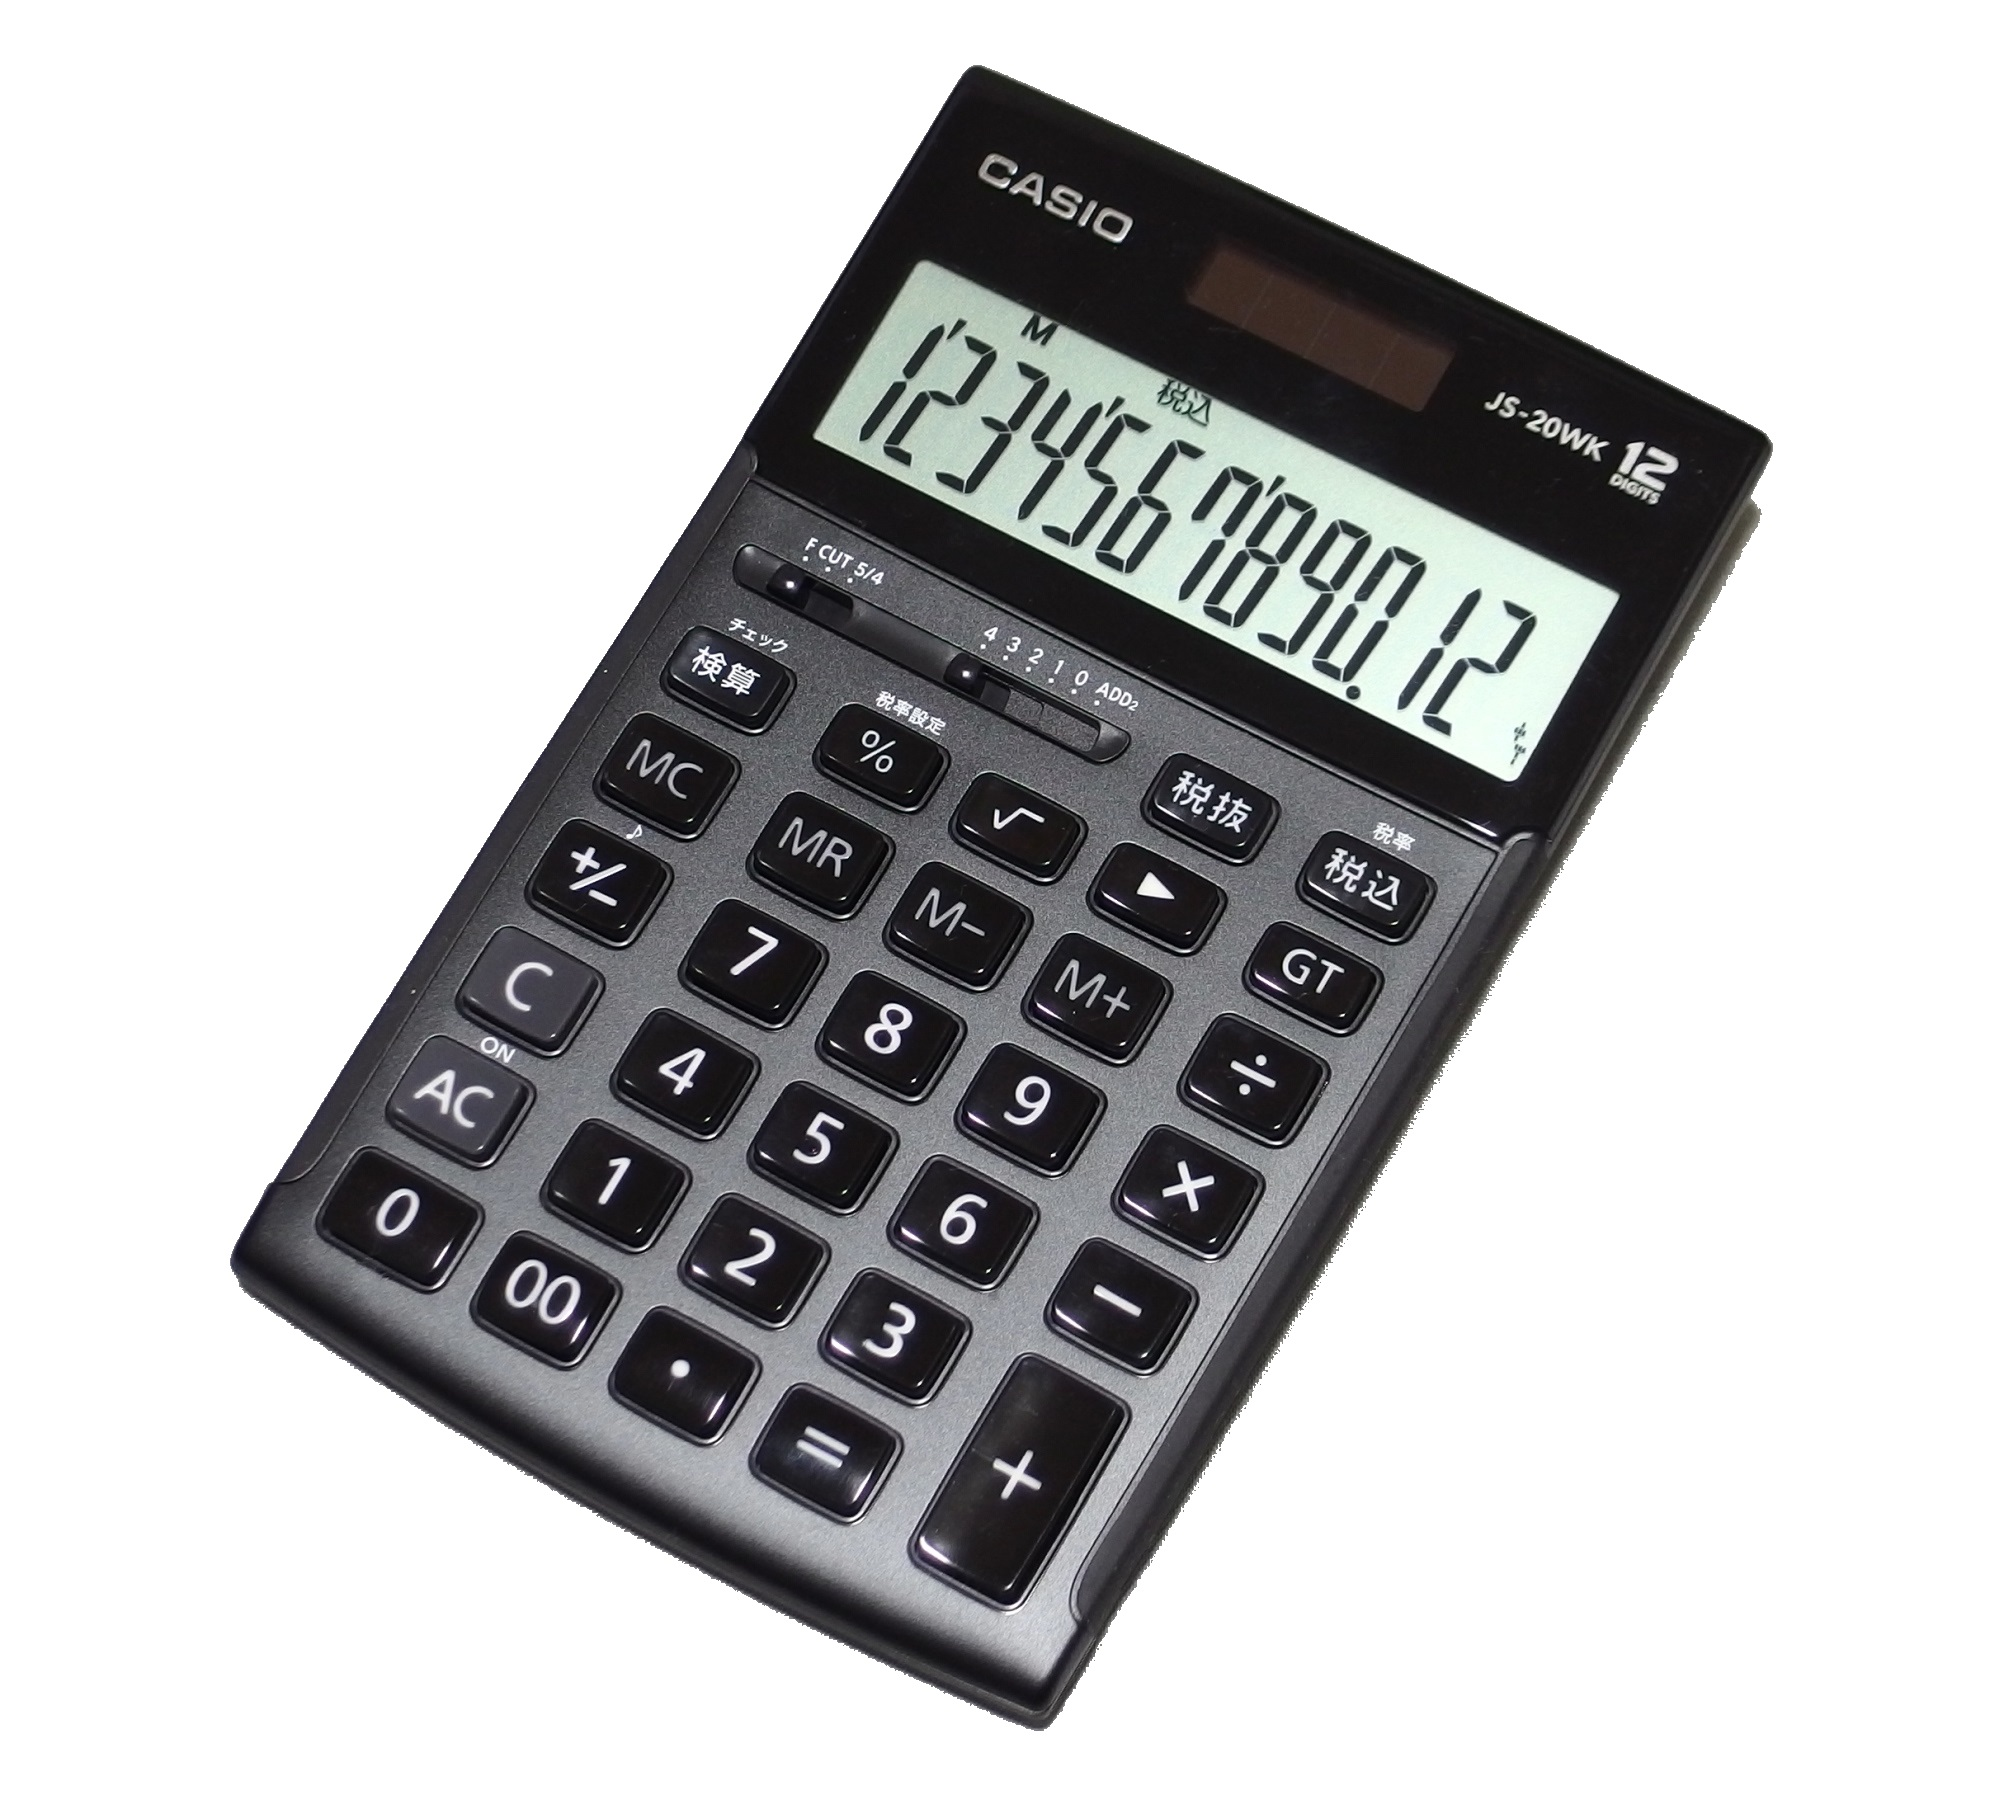
\includegraphics[width=0.7\textwidth]{graphics/0.CasioCalculator.jpg}
  \caption{Casio calculator}
  \label{fig:CasioCalculator}
\end{figure}

The report delves into the \textbf{algorithmic strategies} employed, the \textbf{methodologies of implementation}, and the \textbf{limitations} inherent to this program.
Visual aids such as flowcharts and test case outcomes supplement the narrative, providing clarity and insight into the program's inner workings. The submission adheres rigorously to the evaluation rubric, emphasizing interface friendliness, application functionality, and the quality of the accompanying report. Plagiarism concerns are addressed through originality and adherence to academic integrity standards, ensuring the integrity of the submitted work.